\label{sec:voltage_rails}

In order to power the components  used in this design, three different voltage
levels  (usually referred  to  as voltage  \emph{rails})  are used. These  are
\SI{28}{\volt},  \SI{5}{\volt} and  \SI{3.3}{\volt}.  Each  rail has  specific
requirements concerning  noise, power  and efficiency.   Selecting appropriate
voltage  regulators requires  determining approximate  values for  the maximum
current in each rail.

The most power-hungry  components on the \SI{3.3}{\volt} rail  are the dsPIC33
microcontroller  and LEDs. According  to  the  datasheet \code{TODO:  source},
the microcontroller consumes \SI{0.5}{\milli\ampere\per\mega\hertz}. Since the
microcontroller will be clocked  at \SI{120}{\mega\hertz}, the minimum current
can be calculated using the following equation.

\begin{equation}
    I_{dsPIC} = \SI{0.5}{\milli\ampere\per\mega\hertz} \cdot \SI{120}{\mega\hertz} = \SI{60}{\milli\ampere}
\end{equation}

Each   of  the   four   LEDs  connected   to   the  microcontroller   consumes
\SI{15}{\milli\ampere}. Taking  both the  microcontroller  and  the LEDs  into
account, the total current consumption of the \SI{3.3}{\volt} rail is roughly:
\begin{equation}
    I_{\SI{3.3}{\volt}} = I_{dsPIC} + 4 \cdot \SI{15}{\milli\ampere} = \SI{120}{\milli\ampere}
\end{equation}

The \SI{5}{\volt}  rail supplies  both the \SI{3.3}{\volt}  rail and  the OLED
display with power. According  to its datasheet \code{TODO:  source}, the OLED
display draws a maximum current of \SI{135}{\milli\ampere}. Adding the current
for the \SI{3.3}{\volt} rail yields  an approximate current consumption on the
\SI{5}{\volt} line of:

\begin{equation}
    I_{\SI{5}{\volt}} = I_{\SI{3.3}{\volt}} + \SI{135}{\milli\ampere} = \SI{255}{\milli\ampere}
\end{equation}

Having determined  the current requirements for  each rail, we can  now choose
appropriate methods  to generate  the voltage and  current. The \SI{28}{\volt}
rail is provided by the power supply directly.

The    \SI{5}{\volt}   rail    is   supplied    by   converting    down   from
\SI{28}{\volt}. This  can  either be  accomplished  with  a switch-mode  power
regulator or a linear regulator. The former offers high efficiency at the cost
of jitter  on its output  line, whereas the  latter offers very  smooth output
voltages but  is not very efficient. Therefore,  for converting \SI{28}{\volt}
down to  \SI{5}{\volt}, a switch-mode  regulator is used, otherwise  the power
losses would be inacceptably high due to the larger voltage drop.

Because all  digital circuitry (such  as the microcontroller) operates  on the
\SI{3.3}{\volt} rail,  it is  crucial that  it has  as little  noise/jitter as
possible,  making a  linear regulator  for the  conversion from  \SI{5}{\volt}
to  \SI{3.3}{\volt}  the  preferred  choice. The  reference  voltage  for  the
analog-to-digital  (ADC) and  digital-to-analog (DAC)  conversions is  derived
from the \SI{3.3}{\volt} rail, meaning any  deviations in that rail could lead
to lower accuracy of the device's output voltage. The corresponding circuit is
illustrated  in Figure  \ref{fig:circuit:rails}. The  selected regulator  also
fulfills  the  current  requirement  and  can  supply  a  maximum  current  of
\SI{1}{\ampere}.

\begin{figure}[th!]
    \center
    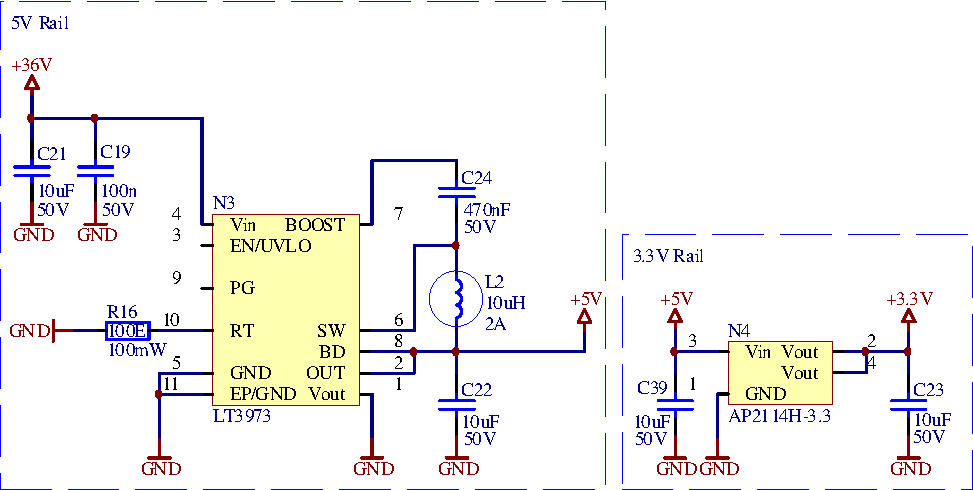
\includegraphics[width=.75\textwidth]{images/circuit/5v-3v-rails.pdf}
    %\caption{Speisung f\"ur 5V mittels Abwertswandler (links) und Speisung f\"ur 3.3V mittels Linearregler (rechts)}
    \caption{Supplying the \SI{5}{\volt} rail via switch-mode regulator (left) and the \SI{3.3}{\volt} rail via linear regulator (right)}
    \label{fig:circuit:rails}
\end{figure}

